\section{Cyclus}

\Cyclus is an agent-based nuclear fuel cycle simulation framework 
\cite{huff_fundamental_2016}, meaning
that each reactor, reprocessing plant, and fuel fabrication plant is modeled as an agent.
A \Cyclus simulation contains prototypes, which are fuel cycle facility models (archetypes) with
pre-defined parameters, that are deployed in the simulation as \texttt{Facility} agents.
Encapsulating the \texttt{Facility} agents are the \texttt{Institution} and \texttt{Region}.
A \texttt{Region} agent holds a set of \texttt{Institution}s. 
An \texttt{Institution} agent can deploy or decommission \texttt{Facility} agents.

Several versions of \texttt{Institution}
and \texttt{Region} agents exist, varying in complexity and purpose \cite{huff_extensions_2014}.
\texttt{DeployInst}, which deploys agents at user-defined timesteps, serves
as the main \texttt{Institution} archetype in this work. All reactor \texttt{Facility} agents,
fuel reprocessing, and fabrication \texttt{Facility} agents
are deployed through \texttt{DeployInst}, while basic fuel cycle \texttt{Facility} agents
such as sink, source, enrichment, and storage facilities are deployed 
through \texttt{NullInst}, which simply deploys \texttt{Facility}
agents at the beginning of the simulation.

At each timestep,
agents make requests for materials or bid to supply them and exchange
with one another. A market-like mechanism called the dynamic resource exchange
\cite{gidden_agent-based_2015} governs the exchanges.
For output analysis, each material resource has a quantity, composition, name, and a unique identifier.

In this work, each nation is represented as a \texttt{Region} agent,
that contains \texttt{Institution} agents, which deploy \texttt{Facility} 
agents according to a user-defined deployment scheme.

Cyclus has multiple advantages over other available
\glspl{NFCS} codes - open-source distribution, modularity,
and extensibility. Its agent-based modeling approach
is ideal for modeling coupled, physics-dependent
supply chain problems common in \glspl{NFC}.
The framework allows for dynamic loading of 
external libraries, which allows the users to plug-and-play
different types of physics models for \gls{NFC}
simulation.

\subsection{Open source distribution}
License agreements and institutional
approval are needed for most \glspl{NFCS} like COSI, DANESS, DESAE, EVOLCODE,
FAMILY21, NFCSim, ORION and VISION \cite{jacobson_verifiable_2010}, challenging
both use and development in an academic setting.
On the other hand, Cyclus relies completely on open source,
free libraries, allowing all users to both use and develop the
Cylcus framework and existing libraries. The open-source distribution
of Cyclus encourages collaboration - any user can propose
improvements or contribute extensions for Cyclus.

\subsection{Modularity and extensibility}
In most modern \glspl{NFCS}, the facilities and their
behaviors (and its fidelity) are confined in the software.
Also, most modern \glspl{NFCS} model
fuel cycles (once-through, continuous reprocessing)
with immutable restrictions to connections between facilities. On the
other hand, Cyclus allows users to plug-and-play various agent models
within the Cyclus framework (shown in figure \ref{fig:core}).
Also, Cyclus relies on a market-based model
for material trades between facilities, so the user can design
any novel fuel cycle. This enables Cyclus to simulate any system analysis
involving multiple connected facilities with physics-based
calculations.


\begin{figure}[htbp!]
	\begin{center}
		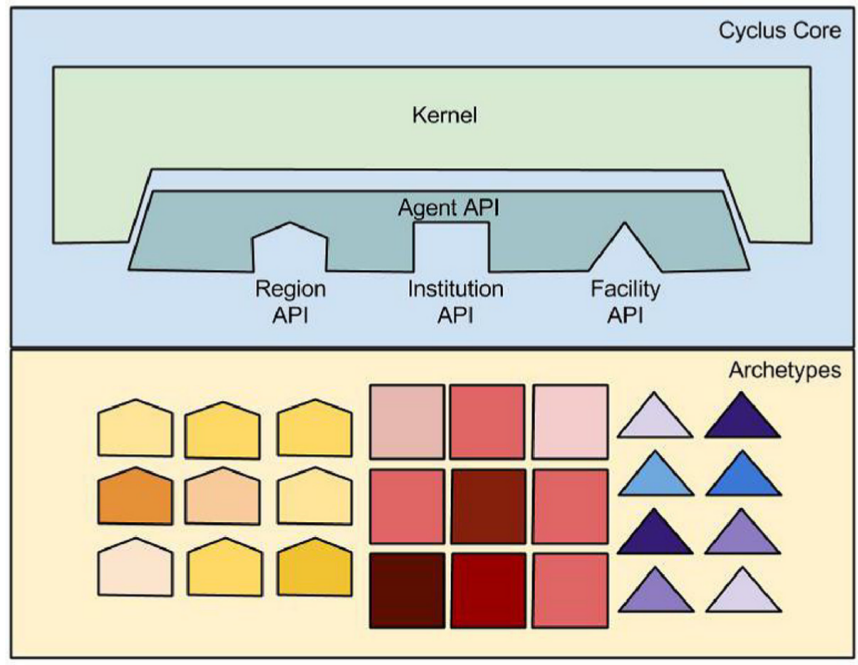
\includegraphics[scale=0.3]{./images/cyclus_core.png}
	\end{center}
	\caption{The Cyclus core provides APIs that the archetypes
			can be loaded into the simulation modularly
			\cite{huff_fundamental_2016}.}
	\label{fig:core}
\end{figure}

Within the Cyclus kernel, the \gls{DRE} connects
the framework and the agents by mediating agent material
offers and requests.
The kernel solves the multicommodity exchange problem
posed by the material offers and requests and executes
the transaction between two agents.

\subsection{Cyclus' fitness for real-world \gls{NFC} transition scenario}
The Cyclus framework and its extension libraries fulfill all the functionalities
specified by Brown et al. \cite{brown_identification_2016}.  Additionally,
its text-based input structure and discrete facility modeling capabilities
allow modeling of real-world, individual reactors. 
Modularity in Cyclus enables adding an \gls{MSR} model without altering Cyclus
itself.
